\section{Dominance Validity Analysis}
\label{sec:dominance_validity_analysis}

This section evaluates whether the generative models produce samples that preserve the intended dominance structure. While Section~\ref{sec:experimental_results} evaluates reconstruction and classification, this section focuses on the central structural question of Gen-MOR: whether generated $P^{+}$ samples remain nondominated and generated $P^{-}$ samples remain dominated under the selected objective subset $S$. In the 50K experiment, DVR is computed using chunked vectorized verification with a reference pool of $10{,}000$ real plans and a generated-sample evaluation cap of $500$ samples per class.

\subsection{Generated $P^{+}$ Validity}
\label{subsec:generated_positive_validity}

Generated $P^{+}$ samples are expected to remain nondominated. For each generated positive sample $\tilde{p}^{+}_i$, the dominance verifier checks whether any plan in the verification pool $\mathcal{V}$ dominates it under the selected objective subset $S$. The positive dominance validity is computed using Eq.~\eqref{eq:positive_dvr}.

The results for generated $P^{+}$ samples are summarized in Table~\ref{tab:positive_dvr_results}.

\begin{table}[H]
\centering
\caption{Positive dominance validity for generated $P^{+}$ samples.}
\label{tab:positive_dvr_results}
\begin{tabular}{|l|c|c|c|}
\hline
\textbf{Model} & \textbf{Evaluated $P^{+}$ Samples} & \textbf{Valid $P^{+}$ Samples} & $\mathbf{DVR^{+}}$ \\
\hline
VAE & $327$ & $287$ & $87.8\%$ \\
CVAE & $500$ & $340$ & $68.0\%$ \\
\hline
\end{tabular}
\end{table}

A high $\operatorname{DVR}^{+}$ means that the model can generate samples that remain on the nondominated side of the dominance structure. In this experiment, the VAE achieves stronger positive dominance validity than the CVAE. The VAE generated $P^{+}$ set achieved $87.8\%$ positive DVR, while the CVAE achieved $68.0\%$. This suggests that VAE-generated positive samples more frequently remain nondominated under the selected MORNP objective subset.

\subsection{Generated $P^{-}$ Validity}
\label{subsec:generated_negative_validity}

Generated $P^{-}$ samples are expected to remain dominated. For each generated negative sample $\tilde{p}^{-}_i$, the verifier checks whether at least one plan in the verification pool $\mathcal{V}$ dominates it under $S$. The negative dominance validity is computed using Eq.~\eqref{eq:negative_dvr}.

The results for generated $P^{-}$ samples are summarized in Table~\ref{tab:negative_dvr_results}.

\begin{table}[H]
\centering
\caption{Negative dominance validity for generated $P^{-}$ samples.}
\label{tab:negative_dvr_results}
\begin{tabular}{|l|c|c|c|}
\hline
\textbf{Model} & \textbf{Evaluated $P^{-}$ Samples} & \textbf{Valid $P^{-}$ Samples} & $\mathbf{DVR^{-}}$ \\
\hline
VAE & $500$ & $227$ & $45.4\%$ \\
CVAE & $500$ & $206$ & $41.2\%$ \\
\hline
\end{tabular}
\end{table}

A high $\operatorname{DVR}^{-}$ means that the model generates samples that correctly remain dominated. In this experiment, negative dominance validity is noticeably lower than positive dominance validity for both models. The VAE achieves $45.4\%$ negative DVR, while the CVAE achieves $41.2\%$. This indicates that generating dominated samples is more difficult than generating nondominated samples in the current Gen-MOR setting.

\subsection{VAE and CVAE DVR Comparison}
\label{subsec:vae_cvae_dvr_comparison}

The VAE and CVAE provide different generation mechanisms. The VAE generates samples from an unconditional latent prior, while the CVAE generates samples conditioned on the target label. Because of this, the CVAE is expected to provide better class control. However, class conditioning does not automatically guarantee dominance validity.

Table~\ref{tab:dvr_comparison} compares the class-specific and overall DVR values. The overall DVR is computed from the evaluated generated samples in Tables~\ref{tab:positive_dvr_results} and~\ref{tab:negative_dvr_results}.

\begin{table}[H]
\centering
\caption{Dominance Validity Rate comparison for generated samples.}
\label{tab:dvr_comparison}
\begin{tabular}{|l|c|c|c|}
\hline
\textbf{Model} & $\mathbf{DVR^{+}}$ & $\mathbf{DVR^{-}}$ & \textbf{Overall DVR} \\
\hline
VAE & $87.8\%$ & $45.4\%$ & $62.2\%$ \\
CVAE & $68.0\%$ & $41.2\%$ & $54.6\%$ \\
\hline
\end{tabular}
\end{table}

\begin{figure}[H]
    \centering
    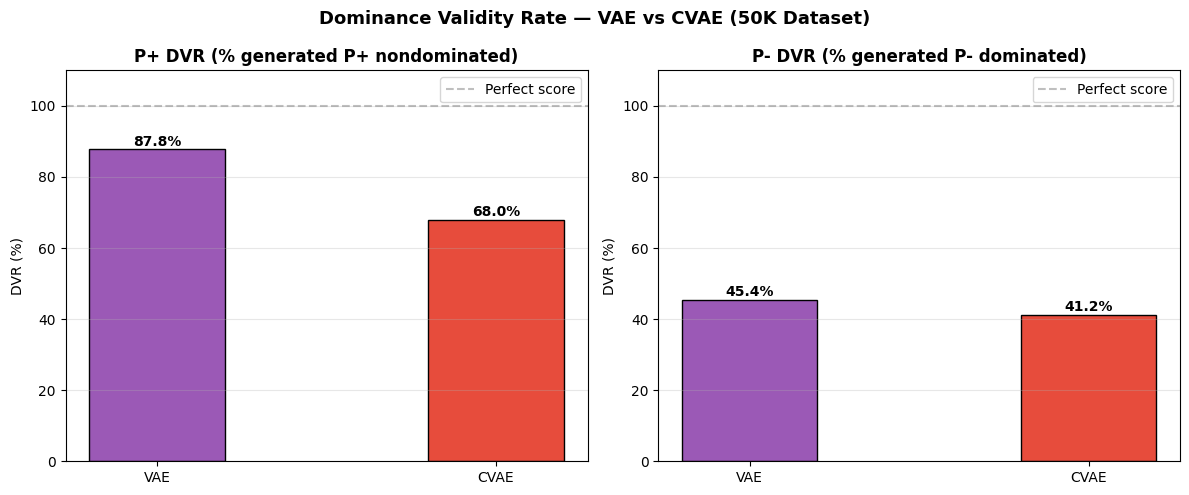
\includegraphics[width=0.90\textwidth]{figures/12_dvr_results.png}
    \caption{Dominance Validity Rate comparison between VAE and CVAE on the Gen-MOR 50K dataset. The left plot shows $P^{+}$ DVR, and the right plot shows $P^{-}$ DVR.}
    \label{fig:dvr_results}
\end{figure}

The comparison in Table~\ref{tab:dvr_comparison} and Fig.~\ref{fig:dvr_results} should be interpreted together with reconstruction and classification performance. Although the CVAE enables class-conditioned generation, it does not outperform the VAE on dominance validity in this experiment. The VAE achieves higher $\operatorname{DVR}^{+}$, higher $\operatorname{DVR}^{-}$, and higher overall DVR. This shows that class conditioning alone is not sufficient to guarantee dominance-preserving generation.

\subsection{Interpretation of DVR Variance}
\label{subsec:dvr_variance_interpretation}

DVR can vary across random seeds because generated samples depend on several stochastic factors. These include network initialization, mini-batch ordering, latent sampling, and the learned geometry of the latent space. Small differences during training may lead to different generated samples, and those generated samples may have different dominance behavior.

This variance is especially important for $P^{+}$ validity. A generated positive sample must avoid being dominated by any other plan in the verification pool. This is a stricter condition than merely resembling the distribution of positive training samples. Similarly, a generated negative sample must be dominated by at least one other plan, which requires the generated point to fall into a dominated region of the objective space.

The single-run DVR results in this section show that VAE performs better than CVAE on both positive and negative DVR. The multi-seed DVR variance is reported in Section~\ref{sec:multi_seed_robustness}. If DVR variance is high across seeds, then the model is not yet stable as a dominance-preserving generator.

\subsection{Dominance Validity vs. Reconstruction Quality}
\label{subsec:dominance_vs_reconstruction}

One of the central observations in Gen-MOR is that reconstruction quality and dominance validity measure different properties. Reconstruction MSE compares an input vector with its reconstructed output. DVR compares a generated vector against other plans using the formal dominance relation.

Therefore, a model can achieve low MSE and still generate invalid samples. This is visible in the current experiment. The CVAE has reconstruction MSE close to the VAE, but it has lower dominance validity. For example, if a generated $P^{+}$ sample is numerically close to the training distribution but is dominated by another plan, then it is invalid under DVR. Similarly, a generated $P^{-}$ sample may look realistic but fail to be dominated by any other plan. This shows that dominance-preserving generation requires more than ordinary distribution learning.

\subsection{Implications for Constraint-Aware Generation}
\label{subsec:constraint_aware_generation_implications}

The DVR results have direct implications for future model design. If VAE or CVAE models achieve reasonable reconstruction and classification performance but weaker DVR, then dominance validity should be incorporated more directly into the learning process. One possible direction is to add a dominance-aware penalty term to the loss function. Another direction is to use rejection sampling or post-generation filtering based on dominance verification.

The broader implication is that Gen-MOR should be treated as a constraint-aware generative modeling problem. The goal is not only to generate samples that look like the training data, but to generate samples that satisfy a relational constraint defined over objective vectors. DVR provides the measurement needed to expose this gap.